\chapter{Specifica e documentazione}
La specifica e la documentazione dei requisiti sono passaggi fondamentali nel
processo di sviluppo di sistemi, assicurando che tutte le parti interessate abbiano
una comprensione chiara delle caratteristiche concordate del sistema.

\subsection*{Dettagli della Specifica}
\begin{itemize}
    \item \textbf{Definizione precisa di tutte le caratteristiche}: Comprende gli
    obiettivi, i concetti, le proprietà del dominio rilevanti, i requisiti del
    sistema, le ipotesi e le responsabilità.
    \item \textbf{Razionale delle opzioni adottate}: Motivazione delle scelte 
    effettuate e argomentazioni per la soddisfazione dei requisiti.
    \item \textbf{Evoluzioni e varianti del sistema}: Discussione sulle possibili 
    evoluzioni e varianti del sistema previste nel tempo.
\end{itemize}

\subsubsection{Organizzazione e Documentazione}
\begin{itemize}
    \item \textbf{Struttura Coerente}: Organizzazione delle informazioni in
    una struttura coerente che faciliti la comprensione e l'utilizzo del documento.
    \item \textbf{Forma di Documentazione}: Preparazione della documentazione in una
    forma comprensibile per tutte le parti coinvolte. Spesso include allegati con costi,
    piani di lavoro e calendari di consegna.
\end{itemize}

\begin{tcolorbox}[colback=orange!5!white,colframe=orange!75!black,title=Documento dei Requisiti]
Il risultato di questo processo
è un documento formale che dettaglia tutti gli aspetti del sistema concordato, servendo
come riferimento principale per lo sviluppo e la manutenzione del sistema.
\end{tcolorbox}
\section{Documentazione libera in linguaggio naturale}
La documentazione libera in linguaggio naturale offre diversi vantaggi
e svantaggi.

\begin{tcolorbox}[colback=green!5!white,colframe=green!75!black,title=Pro della
    documentazione libera]
\begin{itemize}
    \item \textbf{Espressività illimitata}: Il linguaggio naturale permette una
    vasta gamma di espressioni, rendendo la documentazione estremamente versatile.
    \item \textbf{Facilità di comunicazione}: Essendo in linguaggio naturale, la
    documentazione è immediatamente comprensibile senza necessità di formazione specifica.
\end{itemize}
\end{tcolorbox}

\begin{tcolorbox}[colback=red!5!white,colframe=red!75!black,title=Contro della
    documentazione libera]
\begin{itemize}
    \item \textbf{Propensione agli errori e difetti specifici}: La natura illimitata
    del linguaggio naturale lo rende suscettibile a errori di specifica e difetti.
    \item \textbf{Ambiguità intrinseca}: Il linguaggio naturale è naturalmente ambiguo,
    il che può essere dannoso in contesti tecnici. Esempio: interpretazioni errate
    di connettivi logici possono portare a conclusioni sbagliate.
\end{itemize}
\end{tcolorbox}
\section{Documentazione strutturata nel linguaggio naturale}
Tipicamente, un documento dei requisiti non è composto esclusivamente da testo
libero, ma utilizza delle linee guida per strutturare il contenuto in modo coerente
e comprensibile. Qui di seguito sono elencate alcune regole locali per la scrittura
efficace di specifiche in linguaggio naturale.

\begin{itemize}
    \item \textbf{Identifica il pubblico}: Comprendi chi leggerà il documento e scrivi
    di conseguenza per assicurare la chiarezza e la pertinenza del contenuto.
    \item \textbf{Struttura l'informazione}: Dichiara ciò che intendi fare prima di
    farlo, motivando le scelte all'inizio e riassumendo i punti chiave alla fine.
    \item \textbf{Definizione dei concetti}: Assicurati che ogni concetto venga definito
    prima del suo utilizzo nel documento per evitare ambiguità.
    \item \textbf{Chiarimenti continui}: Poni a te stesso domande come ``È comprensibile?",
    ``È sufficiente?" e ``È rilevante?" per mantenere la pertinenza e la qualità del testo.
    \item \textbf{Controllo della complessità}: Evita di includere più di un requisito,
    assunzione o proprietà del dominio in una singola frase. Mantieni le frasi brevi e
    al punto.
    \item \textbf{Linguaggio prescrittivo}: Utilizza ``deve" per indicazioni obbligatorie
    e ``dovrebbe" per quelle desiderabili.
    \item \textbf{Evita gergo tecnico}: Minimizza l'uso di gergo tecnico e acronimi a
    meno che non siano chiaramente definiti o universalmente comprensibili.
    \item \textbf{Esempi illustrativi}: Fornisci esempi suggeriti per chiarire dichiarazioni
    astratte e complesse.
    \item \textbf{Uso di diagrammi}: Include diagrammi per rappresentare relazioni
    complesse tra elementi, facilitando la comprensione visiva delle informazioni.
\end{itemize}

Queste regole sono pensate per migliorare l'efficacia della documentazione mantenendola
accessibile e comprensibile per tutte le parti interessate.

\subsection{Regole locali}
La documentazione dei requisiti di sistema deve seguire regole locali ben definite per garantire coerenza e comprensibilità. Queste regole sono fondamentali per strutturare il contenuto in modo che sia accessibile e tracciabile.
\subsubsection{Uso delle Tabelle Decisionali}
\begin{itemize}
    \item Le tabelle decisionali aiutano a gestire combinazioni complesse di condizioni, offrendo un supporto sistematico e chiarezza nella documentazione dei requisiti.
    \item Questo approccio assicura una completa verifica e un'integrazione logica delle condizioni di input e output.
\end{itemize}

\subsubsection{Modelli di Dichiarazione Standardizzati}
Le tabelle di decisione sono strumenti utilizzati per mappare e implementare le logiche decisionali che coinvolgono condizioni multiple in maniera sistematica e strutturata. Nelle tabelle di decisione, ogni riga rappresenta un insieme di condizioni di ingresso mentre ogni colonna corrisponde a un risultato decisionale specifico. Questo strumento permette agli ingegneri di vedere chiaramente come combinazioni diverse di condizioni d'ingresso influenzino le azioni da intraprendere.

Le condizioni di ingresso possono includere vari fattori come comandi di accelerazione, posizioni relative dei treni, o velocità di ingresso in una stazione, e le azioni corrispondenti possono essere l'attivazione dei sistemi di frenata, l'emissione di allarmi, o altre misure di sicurezza.

\begin{tcolorbox}[colback=green!5!white,colframe=green!75!black,title=Vantaggi delle Tabelle di Decisione]
\begin{itemize}
    \item \textbf{Chiarezza e sistematicità:} Facilitano la comprensione delle relazioni tra cause ed effetti e aiutano a garantire che tutte le possibili situazioni siano considerate.
    \item \textbf{Facilità di manutenzione:} Le modifiche ai criteri o ai procedimenti possono essere implementate aggiornando semplicemente la tabella.
    \item \textbf{Verifica di completezza:} Ogni possibile combinazione di condizioni
    è rappresentata, permettendo un controllo completo su ogni scenario decisionale.
    \item \textbf{Forniscono test di accettazione:} Le tabelle di decisione possono
    essere utilizzate per definire test di accettazione per verificare che il sistema
    soddisfi i requisiti specificati.
\end{itemize}
\end{tcolorbox}

\begin{tcolorbox}[colback=red!5!white,colframe=red!75!black,title=Svantaggi delle Tabelle di Decisione]
\begin{itemize}
    \item \textbf{Scalabilità:} Man mano che il numero di condizioni aumenta, le tabelle diventano esponenzialmente grandi e complesse da gestire.
    \item \textbf{Rigidità:} Possono non adattarsi bene a scenari non previsti e possono richiedere frequenti aggiornamenti per rimanere efficaci in ambienti dinamici.
\end{itemize}
\end{tcolorbox}
\subsubsection{Consigli per i template}
I template standardizzati per la formulazione delle affermazioni sono fondamentali per standardizzare e organizzare la documentazione dei requisiti nei progetti. Di seguito è riportata un'analisi dettagliata dei componenti essenziali di questi template:

Le componenti principali di un template standard per le affermazioni includono:

\begin{itemize}
    \item \textbf{Identificatore:} Serve a nominare l'affermazione in modo intuitivo e, se necessario, gerarchico, facilitando la ricerca e il riferimento incrociato tra affermazioni correlate.
    \item \textbf{Categoria:} Classifica l'affermazione in categorie quali requisiti funzionali o di qualità, assunzioni, proprietà del dominio, definizioni o esempi di scenario. Questa classificazione aiuta ad organizzare le affermazioni in modo logico.
    \item \textbf{Specifica:} Dettaglia la formulazione dell'affermazione seguendo regole stilistiche precise per garantire chiarezza e precisione.
    \item \textbf{Criterio di Adeguazione:} Fornisce criteri per misurare o verificare l'affermazione, essenziali per la validazione e il controllo della qualità.
    \item \textbf{Fonte:} Indica la fonte dell'affermazione per la tracciabilità, collegandola alle evidenze o ai requisiti originali.
    \item \textbf{Razionale:} Spiega il motivo dietro l'affermazione, migliorando la comprensione e facilitando la tracciabilità.
    \item \textbf{Interazione:} Descrive come l'affermazione interagisce con altre affermazioni, inclusi potenziali contributi o conflitti, essenziale per la gestione delle dipendenze.
    \item \textbf{Livello di Priorità:} Stabilisce un livello di priorità per l'affermazione, aiutando nella gestione delle risorse e nella pianificazione del progetto.
    \item \textbf{Stabilità, Livelli di Comunalità:} Aiutano nella gestione del cambiamento e nella valutazione dell'applicabilità dell'affermazione attraverso diverse applicazioni o progetti.
\end{itemize}
\subsubsection{Criteri di Adeguatezza}
I criteri di adeguatamente rendono misurabili le dichiarazioni, quantificando l'estensione
con cui devono essere soddisfatte, essenziali specialmente per la misurabilità dei
requisiti non funzionali (\texttt{NFRs}). Per esempio, le date di riunioni programmate
dovrebbero essere comode per il 90\% dei partecipanti in almeno l'80\% dei casi.

\subsubsection{Documentazione Disciplinata in linguaggio naturale Strutturato}
La documentazione deve seguire regole globali per la strutturazione dei documenti di
requisiti, raggruppando elementi simili come obiettivi del sistema, componenti,
e caratteristiche del software. Questo aiuta a mantenere la documentazione organizzata
e facilmente navigabile.

\subsubsection{Template \texttt{IEEE Std-830} per l'Organizzazione del documento dei Requisiti}
Il template  \texttt{IEEE Std-830} fornisce una struttura standardizzata per organizzare 
il documento dei requisiti,
includendo specifiche per scopo, dominio e altri elementi critici. Questo standard aiuta
le organizzazioni a mantenere una documentazione chiara e conforme alle migliori pratiche
del settore.

\subsubsection{Uso delle Notazioni Diagrammatiche}
Le notazioni diagrammatiche sono utilizzate per completare o sostituire la prosa in
linguaggio naturale. Sono dedicate ad aspetti specifici del sistema (\textit{come è o come sarà})
e sono grafiche per facilitare la comunicazione e fornire una panoramica. Queste notazioni
possono essere semi-formali, includendo:

\begin{itemize}
    \item Dichiarazione di elementi in linguaggio formale (\textit{sintassi, semantica}),
    che permette controlli superficiali sugli elementi del documento dei requisiti e la loro elaborazione
    automatica.
    \item Specifiche informali delle proprietà degli elementi in linguaggio naturale.
\end{itemize}
\section{Documentazione strutturata con l'ausilio di diagrammi}
\subsection{Scope del sistema}
\subsubsection{Context Diagram}
Il diagramma di contesto è uno strumento utile per rappresentare il sistema mediante 
le componenti principali e le relazioni tra di esse. I nodi sono le componenti del sistema,
mentre gli archi rappresentano le relazioni tra di esse. 
\begin{figure}[H]
    \centering
    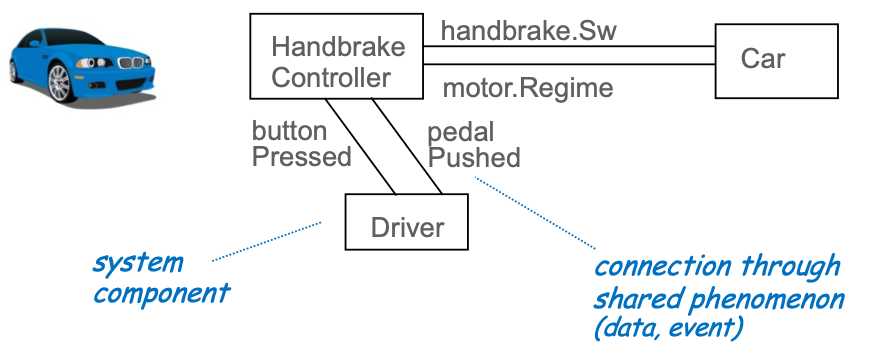
\includegraphics[scale=0.4]{img/context.png}
    \caption{Esempio di Context Diagram}
\end{figure}
\subsubsection{Problem Diagram}
I diagrammi dei problemi sono una forma dettagliata di diagrammi
di contesto che evidenziano i componenti del sistema e le loro interazioni.
Questi diagrammi mostrano chi controlla e monitora i fenomeni condivisi e
indicano i requisiti e i componenti influenzati da essi. 

\begin{figure}[H]
    \centering
    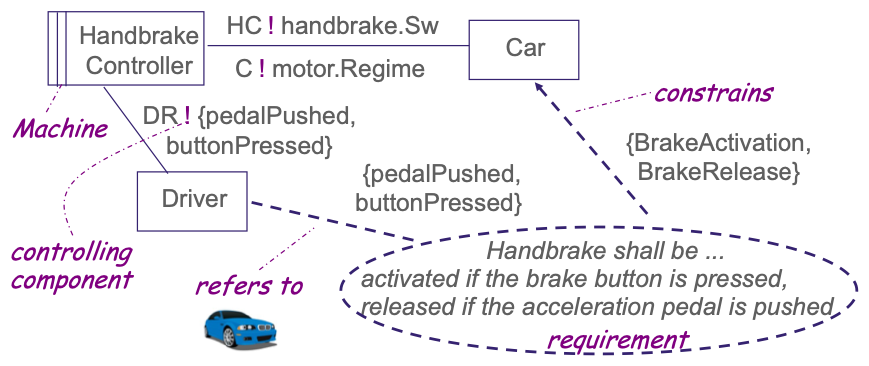
\includegraphics[scale=0.4]{img/problem.png}
    \caption{Esempio di Problem Diagram}
\end{figure}
\subsubsection{Frame Diagram}
I frame diagram sono utilizzati per catturare pattern di problemi frequenti all'interno di un sistema, evidenziando fenomeni tipizzati e componenti tipizzati. Questi diagrammi aiutano a comprendere le interazioni tra i vari elementi del sistema e i requisiti correlati.

\begin{itemize}
    \item \textbf{Fenomeni Tipizzati:}
    \begin{itemize}
        \item \textbf{Causale (C):} Fenomeni che causano effetti diretti.
        \item \textbf{Evento (E):} Fenomeni che rappresentano eventi specifici.
        \item \textbf{Simbolico (Y):} Fenomeni che rappresentano simboli o dati.
    \end{itemize}

    \item \textbf{Componenti Tipizzati:}
    \begin{itemize}
        \item \textbf{Causale (C):} Componenti che causano effetti diretti.
        \item \textbf{Biddable (B):} Componenti che possono essere controllati o influenzati.
        \item \textbf{Lessicale (X):} Componenti che rappresentano dati o informazioni.
    \end{itemize}
\end{itemize}

\begin{figure}[H]
    \centering
    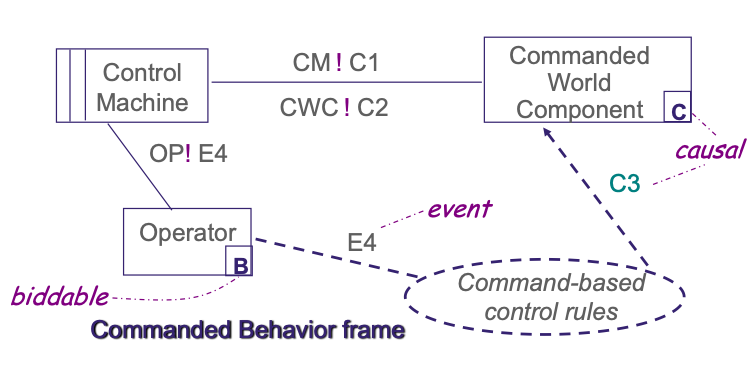
\includegraphics[scale=0.4]{img/frame.png}
    \caption{Esempio di Frame Diagram}
\end{figure}
Un esempio di istanziazione di un frame diagram è il seguente:
\begin{figure}[H]
    \centering
    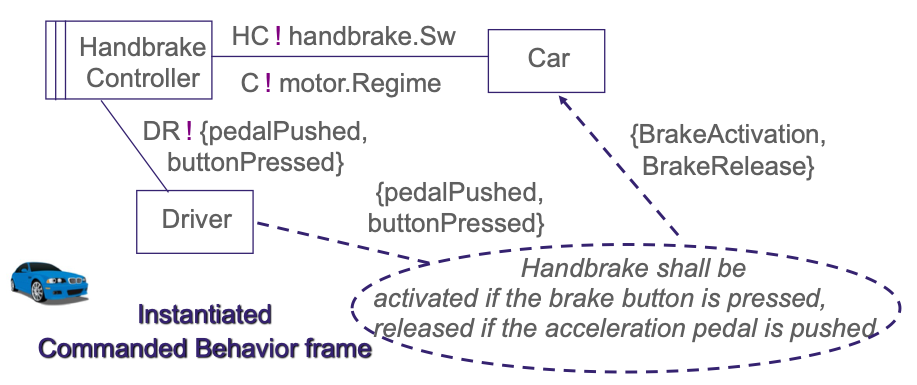
\includegraphics[scale=0.4]{img/instace_frame.png}
    \caption{Esempio di Frame Diagram istanziato}
\end{figure}
\subsection{Diagrammi Entità-Relazione}
I diagrammi Entità-Relazione sono utilizzati per rappresentare le entità e le
relazioni tra di esse in un sistema. Questi diagrammi sono utilizzati per modellare
i dati e le loro interazioni all'interno del sistema, aiutando a definire i requisiti
relativi alla gestione dei dati.

\begin{itemize}
    \item \textbf{Specializzazione delle Entità:} Le entità possono essere
    specializzate in sottoclassi con caratteristiche specifiche (attributi, relazioni).
    Ad esempio, un \textit{ImportantParticipant} eredita attributi e relazioni dalla
    superclass \textit{Participant}, ma può avere attributi aggiuntivi come \textit{Preferences}.
    \item \textbf{Annotazioni dei Diagrammi:} Essenziali per definire con precisione
    gli elementi e evitare errori di specifica. Ad esempio, l'annotazione per
    \textit{Participant} può specificare che è una persona attesa alla riunione in
    un ruolo specifico.
\end{itemize}

\begin{tcolorbox}[colback=red!5!white,colframe=red!75!black,title=Svantaggi dei
    Diagrammi Entità-Relazione]
    Non si riesce a distinguere tra prescrittivi e percettivi.
\end{tcolorbox}
\subsection{Diagrammi \texttt{SADT} (Structured Analytics Design Technique)}
I diagrammi \texttt{SADT} sono utilizzati per catturare attività e dati nel sistema, sia nello stato attuale che in quello futuro. Questi diagrammi si dividono in due categorie principali:

\begin{itemize}
    \item \textbf{Actigram:} Relaziona le attività tramite collegamenti di
    dipendenza dai dati (\textit{input/output}). Mostra come le attività sono correlate
    attraverso i dati che utilizzano e producono.
    \item \textbf{Datagram:} Relaziona i dati tramite collegamenti di dipendenza
    dal controllo (\textit{produttori/consumatori}). Indica come i dati vengono prodotti,
    consumati, validati e le risorse necessarie.
    \begin{itemize}
        \item \textbf{Est:} attività di produzione.
        \item \textbf{Nord:} attività di validazione.
        \item \textbf{Ovest:} attività di consumo.
        \item \textbf{Sud:} risorse necessarie.
    \end{itemize}
\end{itemize}

Nei diagrammi \texttt{SADT}, esiste una dualità dati-attività:
\begin{itemize}
    \item I dati in un actigram devono apparire in un datagram.
    \item Le attività in un datagram devono apparire in un actigram.
\end{itemize}

\begin{tcolorbox}[colback=green!5!white,colframe=green!75!black,title=Vantaggi dei
    Diagrammi \texttt{SADT}]
    \begin{itemize}
        \item Forniscono una chiara visualizzazione delle dipendenze tra attività e dati.
        \item Aiutano a identificare le risorse necessarie e le relazioni di controllo.
    \end{itemize}
\end{tcolorbox}

\begin{tcolorbox}[colback=red!5!white,colframe=red!75!black,title=Svantaggi
    dei Diagrammi \texttt{SADT}]
    \begin{itemize}
        \item Possono diventare complessi e difficili da gestire per sistemi di grandi
        dimensioni.
        \item Richiedono una comprensione approfondita delle attività e dei dati coinvolti.
    \end{itemize}
\end{tcolorbox}

Un esempio di diagramma \texttt{SADT} mostra come le attività di gestione dei vincoli
(\textit{handling constraints}) siano correlate attraverso richieste di meeting,
data range e risorse necessarie. Ogni attività e dato è chiaramente definito
e le loro interazioni sono mappate per garantire la coerenza e la completezza
del sistema.

\subsection{Diagrammi di Flusso dei Dati (\textit{Dataflow Diagrams})}
I diagrammi di flusso dei dati (\texttt{DFD}) sono utilizzati per catturare le operazioni
del sistema collegate dalle dipendenze dei dati. Questi diagrammi sono più semplici
ma meno espressivi rispetto agli actigram.

\begin{itemize}
    \item \textbf{Operazione:} Attività di trasformazione dei dati.
    \item \textbf{Link di Input e Output:} Flussi di dati. Le operazioni richiedono
    dati in entrata per produrre dati in uscita (non flusso di controllo).
    \item \textbf{Regole di Trasformazione dei Dati:} Devono essere specificate nelle
    annotazioni (linguaggio naturale strutturato) o in un altro \texttt{DFD} 
    (raffinamento delle operazioni,
    cf. \texttt{SADT}).
    \item \textbf{Componenti del Sistema e Repositori di Dati:} Origini e destinazioni
    del flusso.
\end{itemize}

\begin{tcolorbox}[colback=green!5!white,colframe=green!75!black,title=Vantaggi dei
    Diagrammi di Flusso dei Dati]
    \begin{itemize}
        \item Semplificano la rappresentazione delle operazioni di trasformazione dei dati.
        \item Facilitano la comprensione delle dipendenze dei dati nel sistema.
    \end{itemize}
\end{tcolorbox}

\begin{tcolorbox}[colback=red!5!white,colframe=red!75!black,title=Svantaggi dei Diagrammi
    di Flusso dei Dati]
    \begin{itemize}
        \item Meno espressivi rispetto agli actigram per rappresentare le operazioni
        complesse.
        \item Richiedono annotazioni dettagliate per specificare le regole di
        trasformazione dei dati.
    \end{itemize}
\end{tcolorbox}

I diagrammi di flusso dei dati sono essenziali per garantire la coerenza e la
completezza del sistema, con ogni attività che deve avere un input e un output,
e tutti i dati devono avere un produttore e un consumatore. Le regole di
consistenza/completa possono essere verificate da strumenti, simili ai diagrammi \texttt{SADT}.
\begin{figure}[H]
    \centering
    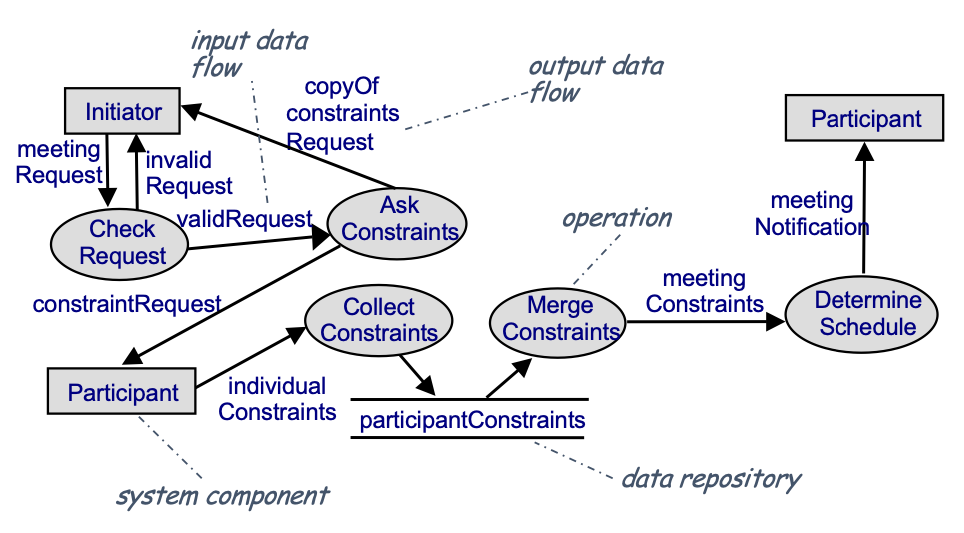
\includegraphics[scale=0.35]{img/dfd.png}
    \caption{Esempio di Diagramma di Flusso dei Dati}
\end{figure}
\subsection{Use Case Diagram}
I diagrammi dei casi d'uso sono utilizzati per catturare le operazioni che devono essere eseguite da un componente del sistema e le interazioni con altri componenti. Questi diagrammi forniscono una vista di insieme semplice ma a volte vaga delle operazioni del sistema.

\begin{itemize}
    \item \textbf{Operazioni del Sistema:} Catturano le operazioni da eseguire
    e le interazioni con altri componenti. Sono introdotti in \texttt{UML} per sostituire i \texttt{DFD}.
    \item \textbf{Annotazioni e Scenari di Interazione:} Necessari per rendere
    precisi i diagrammi dei casi d'uso.
    \item \textbf{Meccanismi di Strutturazione:}
    \begin{itemize}
        \item \texttt{<<include>>}: Specifica una ``sotto-operazione''.
        \item \texttt{<<extend>>} + precondizione: Specifica un'operazione
        ``variante'' in casi eccezionali.
    \end{itemize}
\end{itemize}

\begin{tcolorbox}[colback=green!5!white,colframe=green!75!black,title=Vantaggi
    dei Diagrammi dei Casi d'Uso]
    \begin{itemize}
        \item Forniscono una vista di insieme delle operazioni del sistema.
        \item Facilmente comprensibili anche da stakeholder non tecnici.
    \end{itemize}
\end{tcolorbox}

\begin{tcolorbox}[colback=red!5!white,colframe=red!75!black,title=Svantaggi
    dei Diagrammi dei Casi d'Uso]
    \begin{itemize}
        \item Possono essere troppo vaghi senza annotazioni dettagliate.
        \item Richiedono scenari di interazione per essere completamente utili.
    \end{itemize}
\end{tcolorbox}

I diagrammi dei casi d'uso sono strumenti potenti per la modellazione delle
operazioni del sistema, ma devono essere integrati con annotazioni e scenari
di interazione per garantire una comprensione completa e precisa delle funzionalità
del sistema.
\subsection{Event trace diagrams}
I diagrammi delle tracce degli eventi catturano scenari positivi attraverso
sequenze di interazioni tra istanze dei componenti del sistema. Questi diagrammi
mostrano come le interazioni si svolgono nel tempo.

\begin{tcolorbox}[colback=green!5!white,colframe=green!75!black,title=Vantaggi dei 
    Diagrammi delle Tracce degli Eventi]
    \begin{itemize}
        \item Permettono di visualizzare chiaramente le interazioni tra i componenti 
        del sistema.
        \item Forniscono una sequenza temporale dettagliata degli eventi di interazione.
    \end{itemize}
\end{tcolorbox}

\begin{tcolorbox}[colback=red!5!white,colframe=red!75!black,title=Svantaggi dei 
    Diagrammi delle Tracce degli Eventi]
    \begin{itemize}
        \item Possono diventare complessi con un numero elevato di componenti e interazioni.
        \item Richiedono una comprensione dettagliata delle sequenze di interazione.
    \end{itemize}
\end{tcolorbox}
\subsection{State Machine Diagram}
I diagrammi delle macchine a stati catturano i comportamenti ammissibili dei componenti del sistema. Essi rappresentano la sequenza delle transizioni di stato per gli elementi controllati.

\begin{itemize}
    \item \textbf{Comportamento di un'istanza di componente:} Sequenza di transizioni di
    stato per gli elementi che controlla.
    \item \textbf{Stato della Macchina a Stati:} Insieme di situazioni in cui una variabile
    che caratterizza un elemento controllato ha sempre lo stesso valore. Ad esempio,
    lo stato ``MeetingScheduled'' ha sempre lo stesso valore per ``Date'' e ``Location''.
    \item \textbf{Stati Iniziali e Finali:} Stati in cui l'elemento appare o scompare.
    Gli stati possono avere una certa durata.
    \item \textbf{Transizione di Stato della Macchina a Stati:} Causata da un evento
    associato. Se l'elemento è nello stato di origine e l'evento si verifica, allora passa allo stato di destinazione. Gli eventi sono fenomeni istantanei.
\end{itemize}

\begin{tcolorbox}[colback=green!5!white,colframe=green!75!black,title=Vantaggi dei
    Diagrammi delle Macchine a Stati]
    \begin{itemize}
        \item Permettono di modellare chiaramente i comportamenti ammissibili dei
        componenti del sistema.
        \item Forniscono una rappresentazione dettagliata delle transizioni di stato.
    \end{itemize}
\end{tcolorbox}

\begin{tcolorbox}[colback=red!5!white,colframe=red!75!black,title=Svantaggi dei
    Diagrammi delle Macchine a Stati]
    \begin{itemize}
        \item Possono diventare complessi con un numero elevato di stati e transizioni.
        \item Richiedono una comprensione dettagliata dei comportamenti dei componenti.
    \end{itemize}
\end{tcolorbox}
Per evitare l'esplosione combinatoria di stati è possibile utilizzare gli statecharts,
che permettono di modellare comportamenti complessi in modo più chiaro e conciso.
\begin{figure}[H]
    \centering
    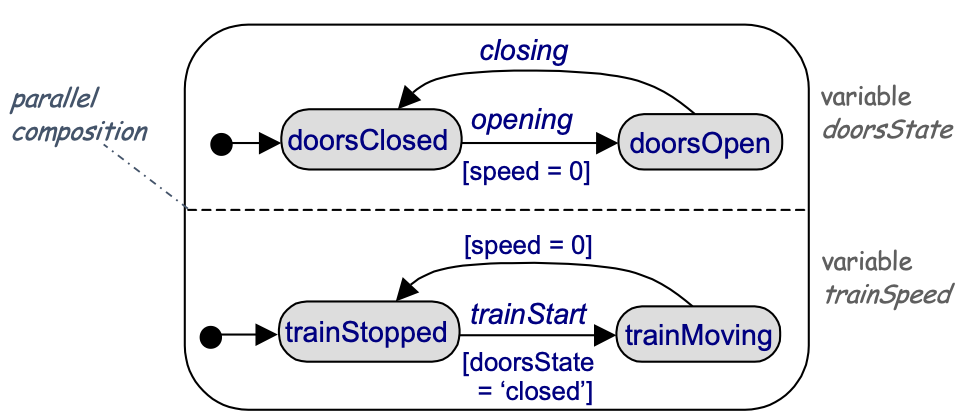
\includegraphics[scale=0.3]{img/statechart.png}
    \caption{Esempio di State Machine Diagram}
\end{figure}
\subsection{\texttt{R-net} Diagram}
Se vogliamo ragionare in termini di stimolo e risposta agli stimoli, 
una versione alternativa è il diagramma \texttt{R-net}, che cattura le relazioni
tra gli stimoli provenienti da un'entità esterna e le risposte generate dal sistema.
\begin{figure}[H]
    \centering
    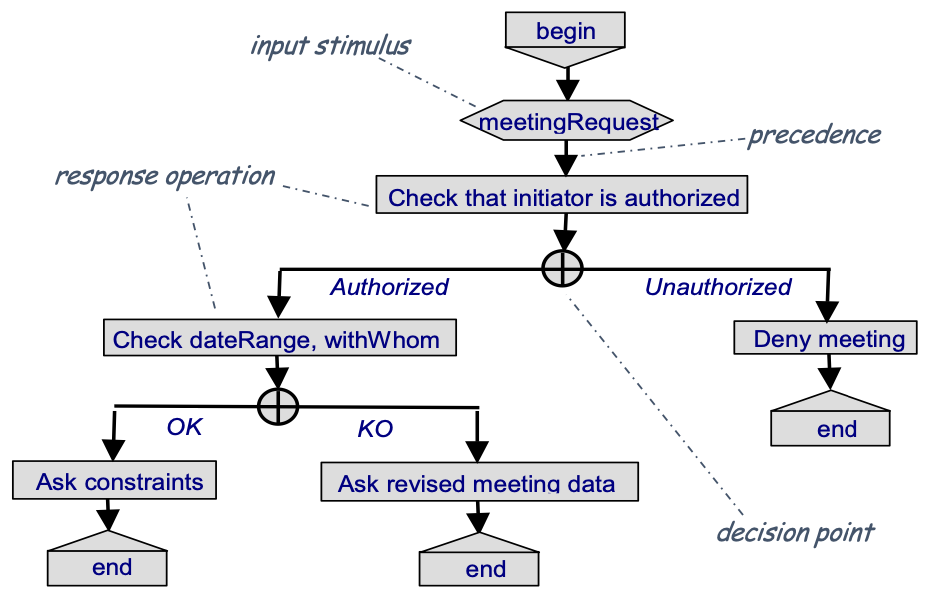
\includegraphics[scale=0.4]{img/rnet.png}
    \caption{Esempio di R-net Diagram}
\end{figure}
\section{Integrare i Diagrammi in un sistema multi-vista}
Avendo a disposizione una varietà di diagrammi per
rappresentare i requisiti del sistema, possiamo integrare i diversi diagrammi dato 
che ciascuno fornisce una prospettiva unica sul sistema. 
Una prima verifica, data dai sistemi automatici, può essere fatta per verificare
la consistenza tra i diagrammi. 

Le inconsistenze che si possono verificare possono essere diverse, tra cui:
\begin{itemize}
    \item tutti i componenti di un problem diagram devono essere presenti
    in un diagramma entità-relazione.
    \item tutti i fenomeni di un problem diagram devono essere presenti
    in un diagramma entità-relazione come un'entità, un attributo o una relazione.
\end{itemize}

Ci sono viste alternative in \texttt{UML} che ci permetto di ragionare, non tanto 
sull'architettura, ma supportano nella fasi di progettazione e validazione dei requisiti,
come ad esempio:
\begin{itemize}
    \item \textbf{Diagrammi delle Classi}: utili per la vista strutturale del sistema.
    \item \textbf{Use Case Diagram}: utile per la vista operazionale del sistema.
    \item \textbf{Sequence Diagram}: utile per la visione degli scenari.
    \item \textbf{State Diagram}: utile per la visione delle state machine.
\end{itemize}

\begin{tcolorbox}[colback=green!5!white,colframe=green!75!black,title=Vantaggi
    dell'ausilio di Diagrammi]
    \begin{itemize}
        \item Sono diversi dalla presentazione in linguaggio naturale, permettendo
        quindi di essere guidati.
        \item Hanno una semantica precisa, non ambigua.
        \item Mezzo di informazione più funzionale per il dialogo con gli stakeholder.
        \item Hanno una struttura grafica che permette di avere una panoramica di 
        alto livello.
        \item Sono facili da capire e da comunicare.
        \item Permettono di fare un'analisi di primo livello e sono supportati da tool.
    \end{itemize}
\end{tcolorbox}
\begin{tcolorbox}[colback=red!5!white,colframe=red!75!black,title=Svantaggi
    dell'ausilio di Diagrammi]
    \begin{itemize}
        \item Il linguaggio semantico può essere vago (\textit{con interpretazioni differenti}).
        \item Spesso vengono formalizzati solo gli aspetti più evidenti e superficiali del
        sistema, lasciando non formalizzate le proprietà dettagliate degli
        elementi, il che può limitare la profondità dell'analisi.
        \item L'analisi automatizzata è limitata.
        \item Si modellano solo aspetti funzionali e strutturali.
    \end{itemize}
\end{tcolorbox}
Le specifiche più formali sono richieste per sistemi \textit{mission critical}.